\begingroup
	\pgfdeclarelayer{background layer}
	\pgfsetlayers{background layer,main}
	\tikzstyle{zero}=[circle,draw=black,fill=white,inner sep=0pt,minimum size=3.5mm]
	\tikzstyle{one}=[circle,draw=black,fill=black,inner sep=0pt,minimum size=3.5mm]
	\tikzstyle{two}=[circle,draw=black,fill=gray,inner sep=0pt,minimum size=3.5mm]
		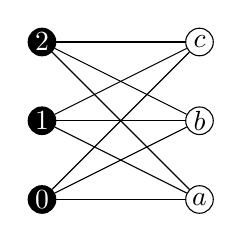
\begin{tikzpicture}
			\foreach \t/\l in {0/a,1/b,2/c}
			{
				\node [white] (\t) at  (1,\t+1) [one] {$\t$};
				\node (\l) at (3,\t+1) [zero] {$\l$};
			}
			\foreach \x in {0,1,2}
			\foreach \l in {a,b,c}
			\draw (\x)--(\l);
		\end{tikzpicture}
	%\label{fig:eg_k_3_3}	
\endgroup